\documentclass[12pt]{report}

\usepackage{blindtext}
\usepackage{listings,xcolor}
%\usepackage[T1]{fontenc}
\usepackage[francais]{babel}
\usepackage[utf8]{inputenc}
%\usepackage[pdftex]{graphicx}
%\usepackage{xcolor}
\usepackage{enumitem}
%\usepackage{listings}
\usepackage{graphicx}
%\usepackage[export]{adjustbox}
%\usepackage{wrapfig}
\usepackage{titlesec}
%\usepackage{hyperref}
%\usepackage{ulem}


\usepackage[a4paper,left=2cm,right=2cm,top=2cm,bottom=2cm]{geometry}
\usepackage{libertine}

\setlength{\parindent}{0cm}
\setlength{\parskip}{1ex plus 0.5ex minus 0.2ex}
%\newcommand{\hsp}{\hspace{20pt}}
\newcommand{\HRule}{\rule{\linewidth}{0.5mm}}


\titleformat{\chapter}[display]
  {\normalfont\bfseries}{}{0pt}{\Large}


\begin{document}

\begin{titlepage}
  \begin{sffamily}
  \begin{center}
    \begin{minipage}{1\textwidth}
    \end{minipage}
    \newline
    \newline
    \newline
    \newline
    \newline
    \newline
    \newline
    \newline
    \newline
    \newline
    \newline
    \textsc{\LARGE Université de Valenciennes et du Hainaut-Cambrésis}\\[4cm]
    \HRule \\[0.4cm]
    { \huge \bfseries M2C - Malware Clustering et Classification\\[0.4cm] }
    \HRule \\[2cm]
    \begin{figure}[htpb]
    \center
	
\includegraphics[width=13cm,height=6.5cm]{img/datascience.png}
    \end{figure}
     \center
        Vincent \textsc{Romé} -
        Axel \textsc{Foulon} -
        Julien \textsc{Dupagny} -
         \center
       	{vrome/afoulon/jdupany}@etu.univ-valenciennes.fr

    \vfill
    {\large — 9 Juin 2018 —}
  \end{center}
  \end{sffamily}
\end{titlepage}
\newpage
\begin{center}
\begin{tabular}{|l|c|l|c|}
   \hline
   \multicolumn{4}{|c|}{HISTORIQUE DES VERSIONS} \\
   \hline
   DATE & VERSION & ÉVOLUTION DU DOCUMENT & RÉDACTEUR \\
   \hline
   9/06/2017 & 0.1 & Version préliminaire & Équipe complète \\
   \hline
\end{tabular}
\end{center}
\tableofcontents

\chapter{Notice légal}
	Le présent document présente et exprime, sauf indication contraire le fruit de la recherche de la réflexion, des idées, et du développement d’une solution pouvant répondre aux besoins et aux spécification du marché de la cyber sécurité en matière de détection de malware. Ce document doit être considéré dès lors comme les points de vue et interprétation des auteurs. Ce document ne reflète pas nécessairement l’état de la technologie la plus récente et pourrait faire l’objet de mises à jours.

	Les sources tierces seront citées, le cas échéant, l’équipe du projet acceptera d’étudier toute requête en cas d’oubli cependant elle ne reste pas responsable du contenu des sources extérieures.
Le dit document a une vocation strictement informative. Tout personne possédant un exemplaire de ce document pourra être tenu responsable de l’usage qu’il pourrait en faire.

\chapter{Introduction}
	Jusqu'à présent les systèmes de détection d'intrusion reposaient traditionnellement sur des signatures générées manuellement par des experts en sécurité, puis nous avons vu apparaître des systèmes permettant de détecter des patterns entre des jeux de données ceci à permis de générer automatiquement ces règles. Aujourd’hui avec l’apparition du “Big Data” des solutions comme le Deep Learning ou  Machine learning sont souvent présentés comme les technologies pouvant révolutionner les systèmes de détections et les performances.
Ces systèmes permettent de générer automatique un modèle de détection à partir de données et leurs capacité à généraliser les événements malveillants permettait en effet de détecter des éléments encore inconnus.
	L’objectif est d’ici comprendre le fonctionnement de ces algorithmes et de les appliquer au milieu de la sécurité informatique. D’exposer les résultats de notre recherche sur la détection de fichier PE (exécutable windows malveillants). Tout en gardant un regard critique sur les résultats et en essayant d’apporter des solution sur l’utilisation de tel algorithme en production.
 
Un modèle de détection supervisé est construit à partir de données labellisées fournies par l’expert : des événements bénins, mais aussi des événements malveillants pour guider le modèle de détection. L’algorithme d’apprentissage va automatiquement chercher les points permettant de caractériser chacune des classes ou de les discriminer pour construire le modèle de détection


\chapter{Abstract}
\chapter{Contexte du projet}
\chapter{Les contraintes}
Il est dès à présent de prendre en compte plusieurs contraintes que nous ne ne devons pas perdre de vu:
\begin{itemize}[label=\textbullet]
	\item Prédiction rapide
	\item Mise à jour périodique du modèle
	\item Interprétable ( Expert puisse comprendre le modèle et l’ajuster)
\end{itemize}

\chapter{Les objectifs}
A travers ce projet nous voulons fournir un solution permettant la classification et une détection via des alorithmes de machine learning de malwares touchant les systèmes d’exploitation Windows de Microsoft.

Nous pourrons découvrir le principe de base d’une analyse statique de fichier malveillant, ainsi que les notions relative au machine learning et la data science pour le traitement de gros flux de données.
Il s'agit d'une application particulière en matière de sécurité informatique des nouveaux algorithmes qui ont le vent en poupe.

L'objectif est qu'a l'issue de ce projet nous soyont en mesure de comprendre les notions de base relative à :
\begin{itemize}[label=\textbullet]
	\item L'analyse de malware
	\item Les algorithmes d'apprentissage automatique
	\item Comprendre le workflow associé à l'utilisation de tel algorithme.
\end{itemize}
A l'issue de ce projet un PoC d'implémentation en python devra être disponible.
Des premiers résultats permettant de conclure sur l'efficacité et la complexité ainsi que les limitions de tel algorithmes appliqué dans le domaine de la sécurité.






\chapter{Le Format PE}
Nous avons décidé de travailler uniquement sur des malwares Windows afin de ne pas compliquer le sujet. Nous sommes partie du constat que la majorité des personnes utilisent ce système d’exploitation.
Le format PE (Portable Executable, executable portable) est le format predominant des fichiers exécutables et des bibliothèques sur les systèmes d'exploitation Windows 32 bits et 64 bits. Ce format est utilisé chez Microsoft pour les pilotes, les programmes mais aussi les DLL et autres fichiers exécutables.  Ce format est dit portable car il peut être porté sous les différents systèmes que Windows NT supporte et il est cross architecture, Il supporte des architectures ( ARM, AMD et Intel).



Les fichiers au format PE peuvent être divisé en plusieurs parties :
\newline\newline\textbf{En-tête MZ-DOS}\newline
Permet à Windows de reconnaître le fichier comme un exécutable. Il contient notamment le magic number MZ.
\newline\textbf{Segment DOS}\newline
Exécuté lorsque le programme est lancé en MS-DOS. La plupart du temps il affiche le message This program must be run under Win32.
\newline\textbf{En-tête PE}\newline
Contient des informations sur le binaire comme sa date de compilation ou encore sa signature.
\newline\textbf{Table des sections}\newline
Un fichier standard PE contient généralement: 
Une section .text ( section de code)
Une ou plusieurs sections de données (.data, .rdata ou .bss)
Des tables de relocation généralement stocker dans la section .reloc


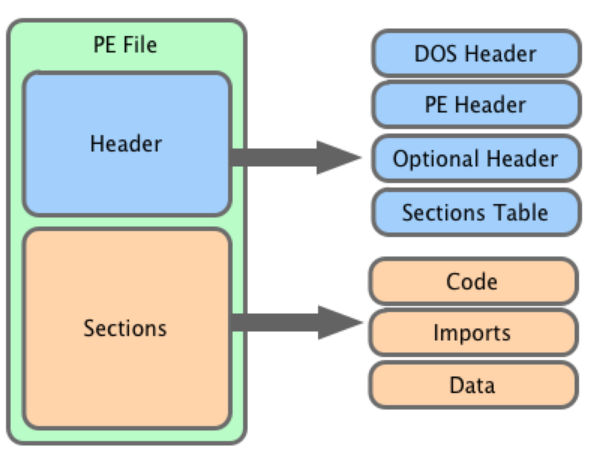
\includegraphics[scale=0.4]{img/FormatPE.png}
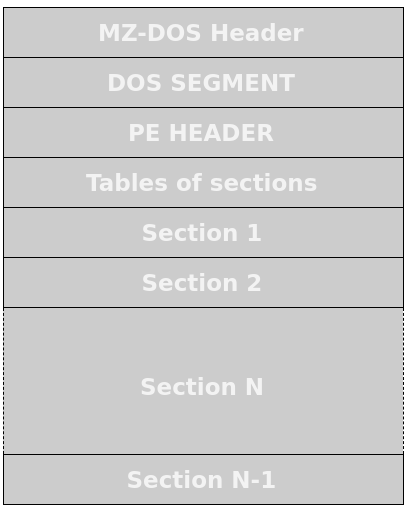
\includegraphics[scale=0.4]{img/FormatPE2.png}
\newpage
Un fichier standard PE contient généralement: 
\begin{itemize}[label=\textbullet]
	\item Une section .text ( section de code)
	\item Une ou plusieurs sections de données (.data, .rdata ou .bss)
	\item Des tables de relocation généralement stocker dans la section .reloc
\end{itemize}

Une autre partie où l'on trouve les sections. Les sections sont en fait des sortes de répertoires dans lesquels sont regroupées des données ayant la même fonctionnalité, du code ou des ressources par exemple, sous un même attribut, qui peut être en lecture seule et écriture par exemple. Il faut donc bien voir ce système de sections qui est présent tout le reste du fichier. Ces sections contiennent le code, quelques informations sur le chargement en mémoire du fichier ou encore des informations de débogage. 


\chapter{Le Fuzzy hashing}
Il s’agit d’un outil dit de fuzzy hashing ceci signifie qu’une valeur de hash qui essaye de détecter le niveau de similarité entre deux fichier au niveau binaire. Ce type de hash est différent d’un hash cryptographique tel que SHA1. Un hash cryptographique standard permet de répondre à la question “ c’est deux fichiers sont-ils identique ?” Un fuzzy hash aussi appelé similarity hash lui est utile pour répondre  à la question “une partie de ce fichier est-elle là même que ce second ?”
Les deux grands algorithme de fuzzy hashing utilisé pour la classification de malware sont :
\begin{itemize}[label=\textbullet]
	\item \textbf{ssdeep : }
	\item \textbf{machocke : } Il s’agit d’un algorithme de fuzzy hashing basé sur le CFG
\end{itemize}

Il peut donc être intéressant d’utiliser ce hash comme feature. Nous n'avons malheureusement pas eu le temps de tester cette possibilité.









\chapter{Implémentation}


\section{Sélections des attribues}
L’étape d’éxtraction d’attributs est quant à elle spécifique à chaque problème de détection

Dans le format PE nous pouvons déjà isoler plusieurs informations intéressant qui nous permettront de faire la différence entre un programme légitime et un malware. 

\textbf{Sections} : le nom, la taille, entropie, ses caractéristiques.\newline
\textbf{Imports}: le nombre de modules, le nombre de symboles, les fonctions\newline
\textbf{Exports}: le nombre de modules, le nombre de symboles, les fonctions
La taille du fichier

Il est nécessaire de définir les attributs à extraire pour représenter les instances sous forme de vecteurs numériques :
\begin{itemize}[label=\textbullet]
	\item Les nombre de Sections
	\item Les noms des sections
	\item L’entropy des sections
	\item les DLL importé
	\item les Fonctions importé
	\item la distribution du jeu d’instruction x86
\end{itemize}

features = ["size_of_file","number_of_sections","median_of_entropy","nb_of_imports","number of exports"]


\section{Format des données - Extraction des features}
Afin de construire notre modèle de détection via du machine learning il est nécessaire de récolter des données d'apprentissage. il faut donc construire un dataset.

Pour constituer notre dataset servira par la suite à l’entraintement de notre algorithme de machine learning, nous allons essayer de générer  une collection de fichier au format JSON.
Dans ces fichiers chaque ligne contiendra un objet JSON. Nous avons tenté  de définir une structure permettant de regrouper suffisamment d’informations.


 Chacun des ces objets inclus les types de données suivant:

Il y a quelques grands principes à respecter lors de la construction du jeu d’apprentissage. Tout d’abord, il doit comporter un nombre suffisant d’instances pour que le modèle de détection soit capable de généraliser correctement les comportements bénin et malveillant.


Exemple de fichier JSON généré pour un fichier:
\lstset{
    string=[s]{"}{"},
    stringstyle=\color{blue},
    comment=[l]{:},
    commentstyle=\color{black},
}


\begin{lstlisting}

{
	"size": 106496,
	"path": "/home/light/Documents/Cours_CDSI/ML/dataset/theZoo/malwares/Binaries/VolatileCedar.Explosion/VolatileCedar.Explosion/0008065861f5b09195e51add72dacd3c4bbce6444711320ad349c7dab5bb97fb",
	"name": "0008065861f5b09195e51add72dacd3c4bbce6444711320ad349c7dab5bb97fb",
	"appeared": "2017-01",
	"label": "-1",
	"hashes": {
		"md5": "d2074d6273f41c34e8ba370aa9af46ad",
		"sha1": "5074ec3ca672f74ea05a7b5f0f52339fbf440f9b",
		"sha256": "0008065861f5b09195e51add72dacd3c4bbce6444711320ad349c7dab5bb97fb"
	},
	"nb_sections": 6,
	"nb_exported_fonctions": 7,
	"nb_imported_fonctions": 95,
	"exported_fonctions": ["CON", "Fdown", "Fdown2", "InetReadF", "_Comp@84", "_PathProcess@4", "_registerapp@8"],
	"imported_fonctions": ["InternetOpenA", "DeleteUrlCacheEntry", "InternetCloseHandle", "InternetOpenUrlA", "InternetReadFile", "CloseHandle", "GetCurrentProcessId", "GetModuleFileNameA", "GetModuleHandleA", "Sleep", "Module32First", "Process32Next", "Process32First", "CreateToolhelp32Snapshot", "InterlockedDecrement", "InterlockedIncrement", "CreateFileA", "WinExec", "TlsSetValue", "GetLocaleInfoW", "HeapSize", "HeapFree", "ExitProcess", "RtlUnwind", "RaiseException", "GetCurrentThreadId", "GetCommandLineA", "GetVersionExA", "HeapDestroy", "HeapCreate", "VirtualFree", "DeleteCriticalSection", "LeaveCriticalSection", "EnterCriticalSection", "HeapAlloc", "VirtualAlloc", "HeapReAlloc", "IsBadWritePtr", "QueryPerformanceCounter", "GetTickCount", "GetSystemTimeAsFileTime", "TlsAlloc", "SetLastError", "GetLastError", "TlsFree", "SetEndOfFile", "TlsGetValue", "GetProcAddress", "SetUnhandledExceptionFilter", "LCMapStringA", "WideCharToMultiByte", "MultiByteToWideChar", "LCMapStringW", "WriteFile", "FlushFileBuffers", "SetFilePointer", "TerminateProcess", "GetCurrentProcess", "SetHandleCount", "GetStdHandle", "GetFileType", "GetStartupInfoA", "FreeEnvironmentStringsA", "GetEnvironmentStrings", "FreeEnvironmentStringsW", "GetEnvironmentStringsW", "UnhandledExceptionFilter", "InitializeCriticalSection", "InterlockedExchange", "VirtualQuery", "LoadLibraryA", "IsBadReadPtr", "IsBadCodePtr", "GetACP", "GetOEMCP", "GetCPInfo", "GetLocaleInfoA", "VirtualProtect", "GetSystemInfo", "GetStringTypeA", "GetStringTypeW", "GetUserDefaultLCID", "EnumSystemLocalesA", "IsValidLocale", "IsValidCodePage", "SetStdHandle", "ReadFile", "RegCreateKeyA", "RegSetValueExA", "RegOpenKeyExA", "RegDeleteValueA", "RegCloseKey", "RegCreateKeyExA", "connect", "URLDownloadToFileA"],
	"imported_libraries": ["WININET.dll", "KERNEL32.dll", "ADVAPI32.dll", "WS2_32.dll", "urlmon.dll"],
	"general": {
		"vsize": 118784,
		"has_debug": 1,
		"exports": 7,
		"imports": 95,
		"has_relocations": 1,
		"has_resources": 1,
		"has_signature": 0,
		"has_tls": 0,
		"symbols": 0,
		"entrypoint": "0x100055dc"
	},
	"header": {
		"coff": {
			"timestamp": 1383637370,
			"machine": "I386",
			"characteristics": ["CHARA_32BIT_MACHINE", "DLL", "EXECUTABLE_IMAGE", "LINE_NUMS_STRIPPED", "LOCAL_SYMS_STRIPPED"]
		},
		"optional": {
			"subsystem": "WINDOWS_GUI",
			"dll_characteristics": [],
			"magic": "PE32",
			"major_image_version": 0,
			"minor_image_version": 0,
			"major_linker_version": 7,
			"minor_linker_version": 10,
			"major_operating_system_version": 4,
			"minor_operating_system_version": 0,
			"major_subsystem_version": 4,
			"minor_subsystem_version": 0,
			"sizeof_code": 65536,
			"sizeof_headers": 4096,
			"sizeof_heap_commit": 4096
		}
	},
	"sections": [{
		"name": ".text",
		"characteristics": 1610612768,
		"vsize": "0xf2eb",
		"size": "0x10000",
		"vaddres": "0x1000",
		"entropy": 6.625413677157515
	}, {
		"name": ".rdata",
		"characteristics": 1073741888,
		"vsize": "0x3a3b",
		"size": "0x4000",
		"vaddres": "0x11000",
		"entropy": 5.043471612579925
	}, {
		"name": ".data",
		"characteristics": 3221225536,
		"vsize": "0x3358",
		"size": "0x1000",
		"vaddres": "0x15000",
		"entropy": 2.7813728969479183
	}, {
		"name": ".SHARDAT",
		"characteristics": 3489660992,
		"vsize": "0x8",
		"size": "0x1000",
		"vaddres": "0x19000",
		"entropy": -0.0
	}, {
		"name": ".rsrc",
		"characteristics": 1073741888,
		"vsize": "0x368",
		"size": "0x1000",
		"vaddres": "0x1a000",
		"entropy": 3.2077393530680016
	}, {
		"name": ".reloc",
		"characteristics": 1107296320,
		"vsize": "0x1630",
		"size": "0x2000",
		"vaddres": "0x1b000",
		"entropy": 5.857932346902008
	}]
}
\end{lstlisting}

\section{Choix technologiques}
Afin d’implémenter notre algorithme de machine learning et d’effectuer des testes, nous avons parcours l’ensemble des technologies disponible aujourd’hui voici celles que nous avons retenue :




\subsection{Redis}
REmote DIctionary Server qui peut être traduit par « serveur de dictionnaire distant » et jeu de mot avec Redistribute1) est un système de gestion de base de données clef-valeur scalable, très hautes performances, écrit en C ANSI et distribué sous licence BSD. Il fait partie de la mouvance NoSQL et vise à fournir les performances les plus élevées possibles. 

Nous aurions pu utiliser d'autres base de données noSQL tel que Spark, MongoDB, très utilisé dans le BigData.


\subsection{SciPy}
SciPy est un projet visant à unifier et fédérer un ensemble de bibliothèques Python à usage scientifique. Scipy utilise les tableaux et matrices du module NumPy.
Cette distribution de modules est destinée à être utilisée avec le langage interprété Python.

pandas
Numpy



\subsection{Scikit-learn}
Nous avons utilisé Scikit-learn est une bibliothèque libre Python dédiée à l'apprentissage automatique. Il existe beaucoup d’autre framework python tel que tensorflow ou encore pytorch. Suite à nos recherches Scikit learn semblait être le mieu documenté et posséder une très grande communauté.


\subsection{LIEF : Library to Instrument Executable Formats}

Pour notre projet comme de nombreux autre nous avons besoin d'analyser les formats exécutables la majorité des projets  ré-implémentent généralement leur propre analyseur de fichier exécutable. Dans les délais impartie étant données que nous ne maîtrisons pas suffisamment bien le format PE. Il n’est pas envisageable de développer de zéro un parser de fichier.
De plus, ces parseurs de fichier sont généralement liés à un langage de programmation particulier.

LIEF : Library to Instrument Executable Formats est un projet initié par QuarksLab qui a pour objectif d’offrir une librairie cross platform qui peut parser et modifier les différents format de fichier ELF, PE, MachO. Cette librairie offre une couche d’abstraction.
Le projet fournit une API Python C/C++


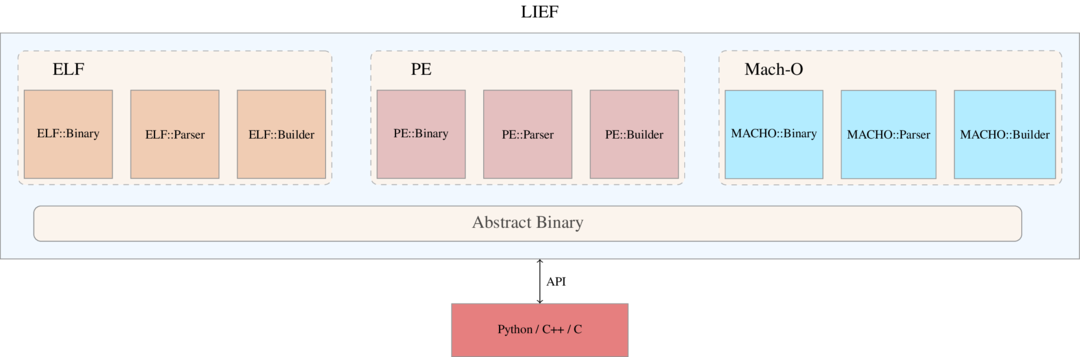
\includegraphics[scale=0.475]{img/archi.png}


\chapter{Nos résultats}
Dans cette partie nous allons essayé de choisir un type de modèle de classification adapté aux contraintes opérationnelles et comparer les résultats de détection obtenues sur différents algorithmes.

\section{K-Means}

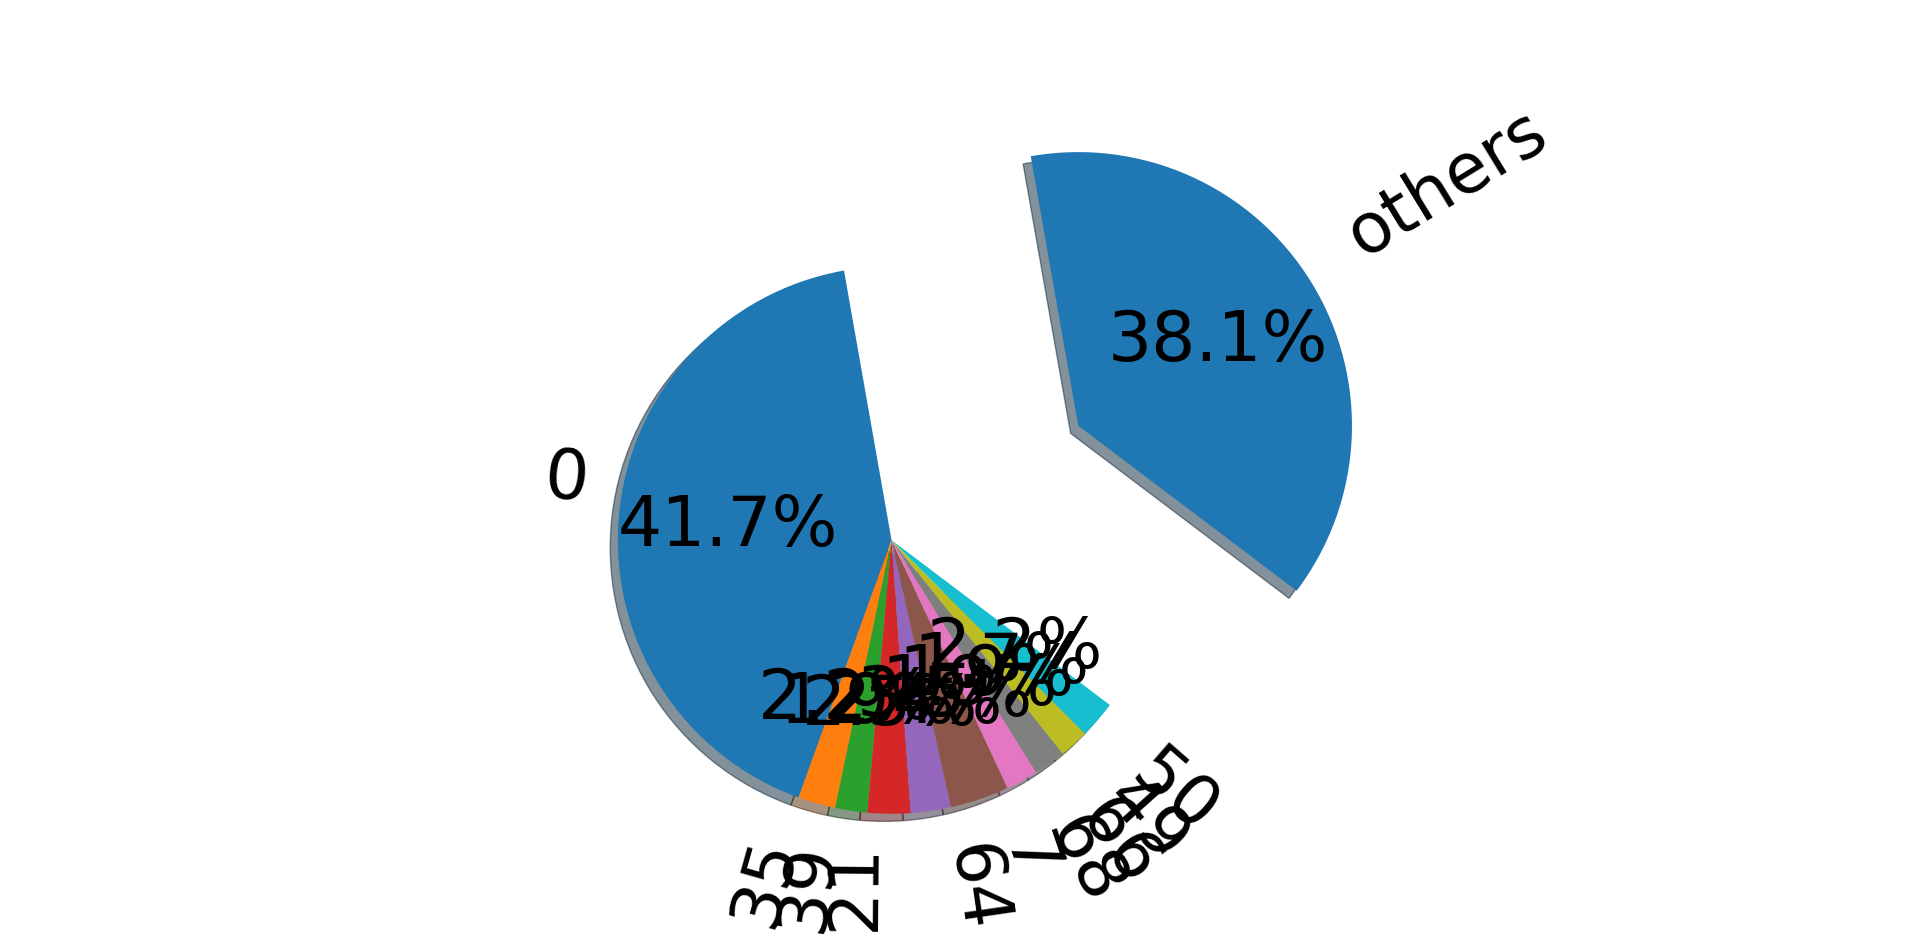
\includegraphics[scale=0.4]{img/results/Kmeans.png}
Ce graphique présente la distribution des malwares du dataset TheZoo que nous avons utilisé.
Nous pouvons noter deux grandes catégories :

Counter({b'EquationGroup': 261, b'EquationGroup.Fanny': 1, b'Backdoor.MSIL.Tyupkin': 1, b'Ransomware.Locky': 1})

Nous remarquons que un gros cluster de malware EquationGroup est majoritairement. Notre jeu n’est pas très homogène et n’est pas représentatif des fichiers pouvant être trouvé dans la nature.

Ces premiers résultats sont intéressant mais pas totalement efficient.
Quand on regarde la phase de normalisation du vecteur, la taille joue un rôle important. Cette feature a tendance à écraser les autres valeurs. Il pourrait donc être intéressant de normaliser en utilisant la valeur max de chaque features. 
La phase de normalisation est très importante.




\chapter{Conclusion}
À travers cet article nous pouvons en conclure :
Le machine learning c’est pas magique, un gros travaille de featuring est nécessaire. Un bon jeu de donnée de départ est aussi très important.
Le multi-architecture et l’extension vers d’autre type de virus que ceux ciblant Windows est facilement envisageable grâce à la library LIEF.
Le machine learning est très utile pour faire un premier filtre afin de catégoriser un gros jeu de données comparé à des algorithmes de fuzzy hashing.
L’utilisation de LightGBM
L’état actuel de nos travaux nous permet de conclure que cette méthode est pertinente et efficace car les résultats obtenus sont déjà très bons alors que de nombreuses pistes sont encore disponibles pour l’améliorer. 
Nous avons implémenté uniquement une solution permettant de faire du clustering nous aimerions nous tourner vers des algorithmes de classification.


\chapter{Définition}
\textbf{Machine Learning : }retrouver des patterns dans un jeu de donnée afin de les regrouper.

\textbf{Classification : }Classer les données dans des catégories prédéfinies. Les algorithmes sont par exemple : decision Tree, Random forest...

\textbf{Clustering : }Regrouper les données dans un ensemble de catégories. Les algorithmes sont par exemple : KMEans HCA DBSCAN...

\textbf{Feature : }Caractéristique  d’un objet utile pour l'algorithme ( les patterns potentiels)

\textbf{Vector of features : } Un tableau de features.

\textbf{Cluster : }Un groupe d’objets décider par l'algorithme

\textbf{Label : } Nom du cluster.

\textbf{CFG : }En informatique, un graphe de flot de contrôle (abrégé en GFC, control flow graph ou CFG en anglais) est une représentation sous forme de graphe de tous les chemins qui peuvent être suivis par un programme durant son exécution.

\textbf{JSON : } JavaScript Object Notation (JSON) est un format de données textuelles dérivé de la notation des objets du langage JavaScript. Il permet de représenter de l’information structurée comme le permet XML par exemple


\end{document}